
\de{ĐỀ THI HỌC KỲ I NĂM HỌC 2022-2023}{Phổ Thông Năng Khiếu}


%Cau 1
\begin{bt}%[0T3B1-4]
Cho hàm số $y=f(x)=\dfrac{1}{\sqrt{2 x-4}}$.
\begin{listEX}
\item Tìm tập xác định của hàm số.
\item Xét tính biến thiên của hàm số đã cho trên tập xác định.
\end{listEX}
\loigiai{
\begin{listEX}
	\item Tìm tập xác định của hàm số.
	\\
	Hàm số xác định khi
	$$
		2x-4>0 \Leftrightarrow x>2
	$$
	Nên tập xác định của hàm số là $ \mathscr{D}=(2;+\infty) $.
	\item Xét tính biến thiên của hàm số đã cho trên tập xác định.
	\\
	Lấy $ x_1, x_2 \in \mathscr{D} $ sao cho $ x_1 \ne x_2 $.
	Xét tỉ số
	\begin{align*}
		T = \dfrac{f(x_2)-f(x_1)}{x_2-x_1}
		&= \dfrac{\dfrac{1}{\sqrt{2x_2-4}}-\dfrac{1}{\sqrt{2x_1-4}}}{x_2-x_1}
		\\
		&= \dfrac{-2}{\sqrt{2x_2-4} \cdot \sqrt{2x_1-4} \cdot \left( \sqrt{2x_2-4}+\sqrt{2x_1-4} \right)}
	\end{align*}
	Ta thấy khi $ x_1, x_2 \in \mathscr{D} $ thì
	\begin{align*}
		&\sqrt{2x_1-4} > 0
		\\
		&\sqrt{2x_2-4} > 0
		\\
		&\sqrt{2x_2-4}+\sqrt{2x_1-4} > 0
	\end{align*}
	nên
	$$
		T = \dfrac{f(x_2)-f(x_1)}{x_2-x_1} < 0 ,\,\forall x_1,x_2 \in \mathscr{D}
	$$
	Vậy $ f(x) $ nghịch biến trên $ \mathscr{D} $.
\end{listEX}
}
\end{bt} 



%Cau 2
\begin{bt}%[0T3B2-1]
Cho hàm số $y=f(x)=a x^2+b x+c$ có đồ thị như hình vẽ
\begin{center}
\begin{tikzpicture}[line join = round, line cap = round,>=stealth,font=\footnotesize,scale=0.7]
\def\xmin{-1.5} \def\xmax{4.5}
\def\ymin{-1.5} \def\ymax{4.5}
\foreach \x in {2} \draw (\x,2pt)--(\x,-2pt) node [above] {$\x$};
\draw[-stealth] (\xmin,0)--(\xmax,0)node[below]{$x$};
\foreach \y in {-1,3} \draw (2pt,\y)--(-2pt,\y) node [left] {$\y$};
\draw[-stealth] (0,\ymin)--(0,\ymax)node[right]{$y$};
\filldraw (0,0)node[below left]{$O$} circle (1.5pt);
\clip (\xmin,\ymin) rectangle (\xmax,\ymax);
\draw[samples=100,domain=\xmin:\xmax,smooth] plot (\x, {(\x)^2-4*(\x)+3});
\draw[dashed](0,-1)--(2,-1)--(2,0);
\end{tikzpicture}
\end{center}
\begin{listEX}
\item Tìm $a$, $b$, $c$.
\item Tìm giá trị lớn nhất và giá trị nhỏ nhất của hàm số đã cho trên đoạn $[0;3]$.
\end{listEX}
\loigiai{
\begin{listEX}
	\item Tìm $a$, $b$, $c$.
	\\
	Gọi $ (P) $ là đồ thị của hàm số đã cho. Dựa vào đồ thị trên, ta thấy $ (P) $ là parabol có đỉnh $ I(2;-1) $ và đi qua điểm $ M(0;3) $ nên ta có hệ phương trình
	$$
		\heva{
		&\dfrac{-b}{2a} = 2\\
		&4a+2b+c=-1\\
		&c=3
		}
		\Leftrightarrow
		\heva{
		&4a+b=0\\
		&4a+2b=-4\\
		&c=3
		}
		\Leftrightarrow
		\heva{
		&a=1\\
		&b=-4\\
		&c=3
		}
	$$
	Vậy $a=1$, $b=-4$ và $c=3$.
	\item Tìm giá trị lớn nhất và giá trị nhỏ nhất của hàm số đã cho trên đoạn $[0;3]$.
	\\
	Dựa vào đồ thị hàm số $ (P) $, ta thấy trên đoạn $ \left[ 0;3 \right] $
	$$
		\heva{
		&y_\text{max} = 3 \quad &\text{khi } x=0
		\\
		&y_\text{min} = -1 \quad &\text{khi } x=2
		}
	$$
\end{listEX}
}
\end{bt}



%Cau 3
\begin{bt}%[0T4K3-1]
Tháp Bánh Ít là một trong số ít những quần thể kiến trúc, văn hoá Chăm còn sót lại ở Việt Nam, được xây dựng vào khoảng cuối thế kỉ XI - đến đầu thế kỉ XII nằm trên ngọn đồi tại thôn Đại Lộc, xã Phước Hiệp, huyện Tuy Phước, tỉnh Bình Định. Theo dòng thời gian, tháp Bánh Ít đã mang trong mình những dấu ấn lịch sử của Vương quốc Chăm Pa cổ đại.\\
Trong một lần di dã ngoại các bạn học sinh trường Phổ thông Năng Khiếu đã thực hiện phép đo ngọn tháp bằng cách đặt hai giác kế (công cụ dùng để đo góc) tại hai điểm $A$,  $B$ trên mặt đất cách nhau $12$ m cùng thẳng hàng với chân $C$ của tháp. Chân của giác kế có chiều cao $h=1{,}3$ m. Gọi $D$ là đỉnh tháp, các điểm $C_1$, $A_1$, $B_1$ thẳng hàng (như hình vē). Các bạn nhận thấy $\widehat{D A_1 C_1}=49^\circ$ và $\widehat{D B_1 C_1}=35^\circ$. Hãy tính chiều cao $C D$ của ngọn tháp.
\begin{flushleft}
\begin{tabular}{ l l  }
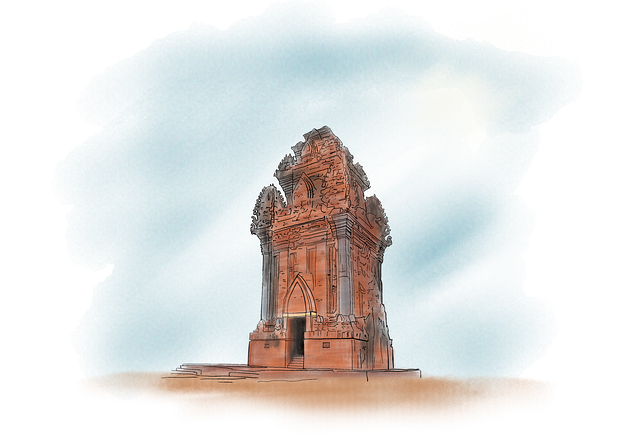
\includegraphics[width=.6\textwidth]{data/thapbanhit_PHOTHONGNANGKHIEU} 
& \begin{tikzpicture}[font=\normalsize,scale=0.5]
%Vẽ Tháp================================================
\coordinate [label=below left:$C$] (C)at(0,0);%chân tháp
\coordinate [label=above:$D$] (D)at($(C)+(0,9)$);%đỉnh tháp
\draw[->,line width=3,>=latex](C)--(D);

\coordinate[label=below:$A$] (A)at(6,0);%điểm A
\coordinate[label=above right:$A_1$] (A1)at(6,2);%điểm A1
\coordinate[label=left:$C_1$] (C1)at(0,2);%điểm C1
\coordinate[label=below:$B$] (B)at(10,0);%điểm B
\coordinate[label=above right:$B_1$] (B1)at(10,2);%điểm B1
\draw (D)--(A1)--(A)(D)--(B1)--(B);
\draw (B1)--(C1);
\draw (C)--($(B)+(2,0)$);
\path (C)--(C1) node[midway,right=0.25] {$1{,}3$ m};
\path (A1)--(B1) node[midway,below] {$12$ m};
\path (A)--(B) node[midway,below] {$12$ m};
%Vẽ góc A
\begin{scope}
\clip (D)--(A1)--(C1);
\draw[opacity=0.7] (A1) circle(1cm)node[shift={(160:10mm)}]{$49^\circ$};
\end{scope}
%Vẽ góc B
\begin{scope}
\clip (D)--(B1)--(C1);
\draw[double,opacity=0.7] (B1) circle(1cm)node[shift={(160:10mm)}]{$35^\circ$};
\end{scope}
\end{tikzpicture}
\end{tabular}
\end{flushleft}
\dapso{$22{,}8$ m.  }
\loigiai{
Xét $ \triangle DA_{1}C_{1} $ vuông tại $ C_{1} $, và $ \triangle DA_{1}B_{1} $ vuông tại $ C_{1} $ ta có
\begin{align*}
	&\dfrac{A_{1}C_{1}}{DC_{1}} = \cot C_{1} \Rightarrow A_{1}C_{1} = DC_{1} \cdot \cot C_{1}
	\\
	&\dfrac{B_{1}C_{1}}{DC_{1}} = \cot B_{1} \Rightarrow B_{1}C_{1} = DC_{1} \cdot \cot B_{1}
\end{align*}
Lại có $ B_{1}C_{1}-A_{1}C_{1}=A_{1}B_{1} $ nên $ DC_{1} \cdot \cot B_{1} - DC_{1} \cdot \cot C_{1} = AB $ suy ra
$$
	DC_{1} = \dfrac{AB}{\cot B_{1} - \cot C_{1}}
	= \dfrac{12\text{ m}}{\cot 35^{\circ} - \cot 49^{\circ}}
	= 21{,}5 \text{ m}
$$
Khi đó
$$
	DC = DC_{1}+C_{1}C = 21{,}5 \text{ m} + 1{,}3 \text{ m} = 22{,}8 \text{ m}
$$
Vậy chiều cao của tháp là $ 22{,}8 \text{ m} $.
}
\end{bt} 

%Cau 4
\begin{bt}%[0T3K2-5][Dự án đề kiểm tra HKI NH22-23- NguyenHuynh]%[PTNK]
	Trong trận chung kết WC2022, L.Messi đã có cơ hội thực hiện cú sút phạt trực tiếp trước khung thành đội Pháp. Các cầu thủ Pháp lập thành hàng rào chắn cách điểm đá phạt $9$ m và cầu thủ cao nhất trong hàng rào là $2$ m. Giả định rằng quỹ đạo quả bóng sau khi Messi thực hiẹn cú sút là một Parabol (như hình vẽ) và nó đạt được chiều cao cực đại là $3$ m sau khi rời chân Messi $14$ m. Hỏi cú đá phạt này của Messi có đưa bóng đi qua điểm cao nhất của hàng rào hay không? Tại sao?
	\begin{center}
		\def\hexagonsize{0.5cm}
		\pgfdeclarepatternformonly
		{hexagons}% name
		{\pgfpointorigin}% lower left
		{\pgfpoint{3*\hexagonsize}{0.866025*2*\hexagonsize}}%  upper right
		{\pgfpoint{3*\hexagonsize}{0.866025*2*\hexagonsize}}%  tile size
		{% shape description
			\pgfsetlinewidth{0.4pt}
			\pgftransformshift{\pgfpoint{0mm}{0.866025*\hexagonsize}}
			\pgfpathmoveto{\pgfpoint{0mm}{0mm}}
			\pgfpathlineto{\pgfpoint{0.5*\hexagonsize}{0mm}}
			\pgfpathlineto{\pgfpoint{\hexagonsize}{-0.866025*\hexagonsize}}
			\pgfpathlineto{\pgfpoint{2*\hexagonsize}{-0.866025*\hexagonsize}}
			\pgfpathlineto{\pgfpoint{2.5*\hexagonsize}{0mm}}
			\pgfpathlineto{\pgfpoint{3*\hexagonsize+0.2mm}{0mm}}
			\pgfpathmoveto{\pgfpoint{0.5*\hexagonsize}{0mm}}
			\pgfpathlineto{\pgfpoint{\hexagonsize}{0.866025*\hexagonsize}}
			\pgfpathlineto{\pgfpoint{2*\hexagonsize}{0.866025*\hexagonsize}}
			\pgfpathlineto{\pgfpoint{2.5*\hexagonsize}{0mm}}
			\pgfusepath{stroke}
		}
		\definecolor{battleshipgrey}{rgb}{0.52, 0.52, 0.51}
		
		\begin{tikzpicture}[line join=round, line cap=round,scale=2,transform shape]
			\clip (-4,-2.5) rectangle (4,2.5);
			
			
			
			\tikzset{cau_thu/.pic={
					\def\T{ 
						(0,2.05)
						..controls +(170:.25) and +(105:.45) ..  (-.3,1.6)
						..controls +(-110:.2) and +(20:0.1) ..  (-.52,1.48)
						..controls +(-130:.1) and +(20:0.1) ..  (-.7,1.4)
						..controls +(-160:.1) and +(20:0.1) ..  (-.9,1.33)
						..controls +(-160:.1) and +(20:0.1) ..  (-1.1,1.3)
						..controls +(-110:.03) and +(10:0.1) ..  (-1.15,1.25)
						..controls +(160:.2) and +(5:.5) ..  (-1.9,1.2)--(-2.1,1.23)
						..controls +(-160:.02) and +(40:.01) ..  (-2.42,1.1)
						..controls +(-110:.05) and +(-170:.01) ..  (-2.3,1.1)
						..controls +(27:.3) and +(20:.2) ..  (-2.17,1.06)
						..controls +(-110:.1) and +(-170:0) ..  (-1.87,1.12)
						..controls +(05:.2) and +(-165:0.25) ..  (-1.13,1.08)--(-1.07,1.07)--(-1.03,1)
						..controls +(15:.37) and +(85:0.2) ..  (-.65,.8)
						..controls +(-80:.1) and +(95:0.2) ..  (-.55,.4)
						..controls +(-120:.2) and +(90:0.3) ..  (-.77,-.05)
						..controls +(-135:.2) and +(35:0.2) ..  (-.95,-.3)
						..controls +(-160:.04) and +(170:0.1) ..  (-.87,-.38)--
						(-1,-.53)
						..controls +(125:.4) and +(-20:0.3) ..  (-1.9,-.4)
						..controls +(110:.2) and +(70:0.2) ..  (-2.22,-.4)
						..controls +(-110:.2) and +(80:0.3) ..  (-2.53,-.7)
						..controls +(-65:.15) and +(-145:0.15) ..  (-2.26,-.67)
						..controls +(25:.2) and +(-179:0.2) ..  (-2,-.6)
						..controls +(45:.1) and +(165:0.25) ..  (-1.05,-.86)
						..controls +(-43:.25) and +(-145:0.25) ..  (-.52,-.69)
						..controls +(-55:.15) and +(-135:0.1) ..  (-.27,-.55)
						..controls +(-55:.15) and +(-135:0.1) .. (-.15,-.63)
						..controls +(-35:.15) and +(125:0.1) .. (.42,-1)
						..controls +(-105:.33) and +(115:0.25) .. (1,-1.75)
						..controls +(-105:.3) and +(-175:0.25) .. (1.3,-2)
						..controls +(5:.1) and +(-95:0.2) .. (1.7,-1.9)
						..controls +(110:.1) and +(-30:0.35) .. (1.25,-1.75)
						..controls +(120:.05) and +(5:0.05) .. (1.15,-1.7)
						..controls +(130:.4) and +(-45:0.05) .. (.7,-.85)
						..controls +(75:.18) and +(-60:.16) .. (.27,-.34)
						..controls +(10:.05) and +(-30:.1) .. (.15,-.18)
						..controls +(120:.05) and +(-70:.1) .. (.05,0)--(.08,0.25)--(.23,0.1)
						..controls +(-95:.12) and +(110:.13) .. (.43,-.16)
						..controls +(35:.1) and +(-120:.1) .. (.4,0)
						..controls +(-25:.2) and +(-170:.1) .. (.68,-.16)
						..controls +(125:.2) and +(-25:.1) .. (.3,.18)
						..controls +(140:.23) and +(-45:.1) .. (.1,.45)
						..controls +(85:.06) and +(-85:.04) .. (.09,.67)
						..controls +(65:.1) and +(-135:.04) .. (.11,.82)
						..controls +(75:.17) and +(-125:.1) .. (-.052,1.35)
						..controls +(-20:.07) and +(-100:.06) .. (.046,1.39)
						..controls +(50:.01) and +(-38:.025) .. (.096,1.45)--(.13,1.45)
						..controls +(110:.03) and +(-175:.04) .. (.18,1.5)
						..controls +(120:.03) and +(-165:.04) .. (.23,1.65)
						..controls +(85:.03) and +(-95:.04) .. (.24,1.76)
						..controls +(25:.08) and +(-23:.075) .. (.16,1.974)
						..controls +(125:.08) and +(5:.06) .. cycle
						;}
					
					\draw \T;
					\fill[battleshipgrey] \T;
			}}
			\tikzset{cau_thu_2/.pic={
					\def\C{ 
						(.65,1.73)
						..controls +(-173:.3) and +(105:.1) ..  (.44,1.43)--(.41,1.4)
						..controls +(-160:.2) and +(-10:.1) ..  (.1,1.39)
						..controls +(-160:.25) and +(10:.1) ..  (-.31,1.3)
						..controls +(-80:.05) and +(20:.1) ..  (-.5,1.23)
						..controls +(-135:.2) and +(60:.2) ..  (-.8,.8)
						..controls +(160:.15) and +(-20:.2) ..  (-1.05,.72)
						..controls +(-160:.1) and +(-130:.2) ..  (-.73,.72)
						-- (-.56,.9)
						..controls +(40:.1) and +(-130:.2) ..  (-.35,1.1)
						..controls +(-20:.03) and +(-160:.03) ..  (-.27,1.1)--(-.26,1.05)--(-.15,1.05)--(-.25,.7)
						..controls +(-110:.2) and +(50:.1) .. (-.6,.35)
						..controls +(-110:.2) and +(170:.1) .. (-.5,.32)
						..controls +(-120:.4) and +(80:.4) .. (-.65,-.45)--(-.6,-.45)--(-.65,-.67)
						..controls +(-160:.4) and +(40:.4) .. (-1.4,-1.2)
						..controls +(-165:.2) and +(140:.4) .. (-1.37,-1.55)
						..controls +(-85:.2) and +(-160:.1) .. (-1.1,-1.68)
						..controls +(125:.4) and +(-85:.1) .. (-1.2,-1.35)
						..controls +(110:.15) and +(-115:.2) .. (-.5,-.85)
						..controls +(10:.05) and +(-85:.05) .. (-.37,-.77)
						..controls +(20:.05) and +(-120:.05) .. (-.23,-.57)--(-.19,-.6)--(0,-.22)--(.18,-.32)--(.23,-.26)--(.4,-.27)
						..controls +(-160:.35) and +(30:.35) .. (-.25,-.8)
						..controls +(-150:.4) and +(160:.1) .. (-.2,-1.07)
						..controls +(-45:.4) and +(-40:.2) .. (.05,-1.1)
						..controls +(125:.1) and +(-85:.1) .. (.03,-.9)
						..controls +(110:.15) and +(-115:.2) .. (.67,-.4)
						..controls +(20:.1) and +(-35:.1) .. (.74,-.2)
						..controls +(130:.15) and +(-35:.15) .. (.15,.32)
						..controls +(45:.15) and +(-135:.05) .. (.47,.7)
						..controls +(15:.05) and +(165:.15) .. (.84,.73)
						..controls +(45:.05) and +(95:.15) .. (1,.71)
						..controls +(-10:.05) and +(-15:.15) .. (.9,.9)--(.77,.84)--(.54,.88)
						..controls +(30:.05) and +(-45:.1) .. (.6,1.2)
						..controls +(-45:.1) and +(-55:.05) .. (.74,1.2)
						..controls +(-25:.06) and +(-30:.04) .. (.76,1.25)
						..controls +(-25:.1) and +(-30:0) .. (.8,1.3)--(.86,1.3)--(.84,1.4)--(.88,1.43)%mũi
						..controls +(90:.15) and +(5:.2) .. cycle
						;}
					
					\draw \C;
					\fill[battleshipgrey] \C;
			}}
			\tikzset{khung_thanh/.pic={
					\def\K{ 
						(3,-1)--(3,.3)--(3.3,.3)--(3.5,-1) (3.05,-1)--(3.05,.3) (3.2,.3)--(3.2,-1) (3.35,-.1)--(3.35,-1) (3.05,.1)--(3.33,.1) (3.05,-.1)--(3.36,-.1) (3.05,-.3)--(3.39,-.3) (3.05,-.5)--(3.42,-.5) (3.05,-.7)--(3.45,-.7) (3.05,-.9)--(3.48,-.9);}
					\draw \K;
			}}
			
			\tikzset{bong/.pic={
					\def\B{ 
						(0,0) circle (.7cm);}
					\draw[pattern=hexagons,scale=.8] \B;
			}}
			
			\def\xmin{-3.2} \def\xmax{4}
			\def\ymin{-1.5} \def\ymax{2} 
			\draw[->] (\xmin,-1)--(\xmax,-1) node [above left]{\tiny $x$};
			\draw[->] (-2.5,\ymin)--(-2.5,\ymax) node [left]{\tiny $y$};
			\node at (-2.5,-1) [below left]{\tiny $O$};
			\node at (-.1,.43) [above]{\tiny $B$};
			\draw[fill=black] (-.1,.43) circle (.5pt);
			\node at (-.1,-1) [below]{\tiny $9$};
			\draw[fill=black] (-.1,-1) circle (.5pt);
			\node at (3,-1) [below]{\tiny $20$};
			
			\draw[fill=black] (-2.5,0.04) circle (.5pt);
			\node at (-2.5,0.04) [left]{\tiny $2$};
			
			\draw[fill=black] (-2.5,.55) circle (.5pt);
			\node at (-2.5,.55) [left]{\tiny $3$};
			\draw[dashed] (-2.5,.55)--(1.2,.55) (-.1,.43)--(-.1,-1);
			%\draw[fill=black] (-2.5,.02) circle (.3pt);
			%\node[fill=black,rectangle,draw] (.2) at (-2.2,-.5) {};
			\draw (-2.5,-1)..controls +(65:1) and +(165:3) ..  (3,.3);
			\path (-2.5,-.5)pic[scale=.25]{cau_thu}
			(0,-.5)pic[scale=.28,rotate=170,yscale=-1]{cau_thu_2}
			(0,0)pic[scale=1]{khung_thanh} (1.3,.56)pic[scale=.3]{bong};
			
		\end{tikzpicture}
	\end{center}
	\loigiai{Giả sử $(P):y=ax^2+bx+c$. Từ giả thiết, ta có hệ phương trình sau:
		\[\heva{&a\cdot0^2+b\cdot0+c=0\\&a\cdot14^2+b\cdot14+c=3\\&\dfrac{-b}{2a}=14}\Leftrightarrow\heva{&c=0\\&196a+14b+c=3\\&28a+b=0} \Leftrightarrow\heva{&a=\dfrac{-3}{196}\\&b=\dfrac{3}{7}\\&c=0.}\]\\
		Vậy $(P)\colon y=-\dfrac{3}{196}x^2+\dfrac{3}{7}x$.\\
		Độ cao của quả bóng tại vị trí $x=9$ là $y=\dfrac{-3}{196}\cdot9^2+\dfrac{3}{7}\cdot9=\dfrac{513}{196} \approx 2,62$.\\
		Vậy bóng vượt qua được rào cản, vì chiều cao quả bóng khi đó là $2{,}62$ m.}
\end{bt}



%Cau 5
\begin{bt}%[0T5K4-3][Dự án đề kiểm tra HKI NH22-23- NguyenHuynh]%[PTNK]
	Cho tam giác $A B C$ có $A B=2$, $A C=2 \sqrt{2}$ và $\widehat{B A C}=135^\circ$. Gọi $M$ là điểm nằm trên cạnh $B C$ sao cho $B C=3 CM$.
	\begin{listEX}
		\item Tính $\overrightarrow{A B} \cdot \overrightarrow{A C}$. Tính độ dài đoạn thẳng $B C$.
		\item Biểu diễn $\overrightarrow{A M}$ theo $\overrightarrow{A B}$, $\overrightarrow{A C}$. Tính $AM$.
		\item Gọi $N$ là điểm thỏa mãn $\overrightarrow{A N}=x \overrightarrow{A C}$, $x \in \mathbb{R}$. Tìm $x$ sao cho $B N \perp A M$.
	\end{listEX}
	\loigiai{ 
		\begin{listEX}
			\item $\overrightarrow{AB} \cdot \overrightarrow{AC}=AB\cdot AC\cdot\cos \widehat{BAC}=2\cdot2\sqrt{2}\cdot\cos 135^{\circ}=-4$.\\
			Ta có
			\begin{eqnarray*}
				BC^2&=&\overrightarrow{BC}^2=\left(\overrightarrow{AC}-\overrightarrow{AB}\right)^2
				\\&=&AC^2-2\overrightarrow{AB}\cdot\overrightarrow{AC}+AB^2
				\\&=&20
			\end{eqnarray*}
			Suy ra $BC=2\sqrt{5}$.
			\item Ta có $BC=3 CM \Rightarrow \overrightarrow{BC}=-3 \overrightarrow{CM}$.
			\begin{eqnarray*}
				BC=3 CM &\Rightarrow&\overrightarrow{BC}=-3 \overrightarrow{CM}
				\\&\Rightarrow& \overrightarrow{AC}-\overrightarrow{AB}=-3\overrightarrow{AM}+3\overrightarrow{AC}\\&\Rightarrow&	\overrightarrow{A M}=\dfrac{1}{3}\overrightarrow{AB}+\dfrac{2}{3}\overrightarrow{AC}.
			\end{eqnarray*}
			Ta có
			\begin{eqnarray*}
				AM^2 &=&\overrightarrow{AM}^2=\left(\dfrac{1}{3}\overrightarrow{AB}+\dfrac{2}{3}\overrightarrow{AC}\right)^2
				\\&=& \dfrac{1}{9}AB^2+\dfrac{4}{9}\overrightarrow{AB}\cdot\overrightarrow{AC}+\dfrac{4}{9}AC^2\\&=&\dfrac{20}{9}.
			\end{eqnarray*}
			Suy ra $AM=\dfrac{2\sqrt{5}}{3}$.
			\item Ta có $\overrightarrow{BN}=\overrightarrow{AN}-\overrightarrow{AB}=x\overrightarrow{AC}-\overrightarrow{AB}$.\\
			Ta lại có 
			\begin{eqnarray*}
				BN \perp AM &\Leftrightarrow&\overrightarrow{BN} \cdot \overrightarrow{AM} =0
				\\&\Leftrightarrow&\left(x\overrightarrow{AC}-\overrightarrow{AB}\right)\cdot \left(\dfrac{1}{3}\overrightarrow{AB}+\dfrac{2}{3}\overrightarrow{AC}\right)=0
				\\&\Leftrightarrow&
				\Leftrightarrow
				\dfrac{2x}{3}\cdot AC^2 - \dfrac{1}{3}AB^2 +\left(\dfrac{x}{3}-\dfrac{2}{3}\right) \overrightarrow{AB} \cdot \overrightarrow{AC}=0
				\\&\Leftrightarrow&	\dfrac{2x}{3}\cdot8 - \dfrac{1}{3}\cdot4 +\left(\dfrac{x}{3}-\dfrac{2}{3}\right) (-4)=0 \\&\Leftrightarrow&	
				x=\dfrac{-1}{3}.
			\end{eqnarray*}
		\end{listEX}
	}
\end{bt}
